\documentclass[11pt]{report}

\usepackage[left=2cm, right=2cm, top=2cm]{geometry}
\usepackage[spanish]{babel}
\usepackage[utf8]{inputenc}
\usepackage{amsmath}
\usepackage{amssymb}
\usepackage{graphicx}
\graphicspath{ {images/} }

\begin{document}

%Macros generales
\newcommand{\BP}[1]{\bigg( #1 \bigg)} %Paréntesis demasiado grandes
\newcommand{\Bp}[1]{\Big( #1 \Big)} %Paréntesis muy grandes
\newcommand{\bp}[1]{\big( #1 \big)} %Paréntesis grandes pero no tanto

%Macros específicos
\newcommand{\tsint}[1]{\int_0^{#1}} %Integral para el ejercicio 37, lím. inf. 0.

\begin{center}
		\textsc{\huge Matemáticas para las \\Ciencias Aplicadas III \\ Tarea 2\\}
		\textbf{Alan Arteaga, Alma Sánchez, Jerónimo Almeida}
\end{center}

\textbf{El "cuaderno" dónde se resuelven los problemas evaluados en un CAS se encuentran
		en la siguiente liga: }

\textbf{Anton-Bivens-Davis} \\

\textbf{Sección 14.2} \\

\textbf{37-38} Use double integration to find the volume of the solid. \\

\textbf{37.} \\

\begin{figure}[h]
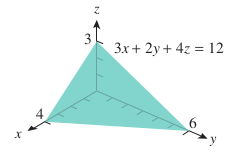
\includegraphics[scale=0.5]{img1.png}
\centering
\end{figure}

Tenemos que integrar
\[\int_0^4 \int_0^{6-3x/2}\left( 3- \frac{3x}{4}- \frac{y}{2} \right) dy dx\]
Comenzamos a integrar respecto a $y$, por lo que pasa como constantes $(3- \frac{3x}{4})$ multiplicado por $y$, entonces :
\[\int_0^4 y \left( 3- \frac{3x}{4}\right)- \frac{y^2}{4} \vert_0^{6-3x/2} dx\]
Evaluamos:
\[\int_0^4 \left(6 - \frac{3x}{2} \right)\left( 3- \frac{3x}{4}\right)- \frac{\left(6 - \frac{3x}{2} \right)^2}{4} dx = 12\]

\textbf{Sección 14.5} \\

\textbf{37.} Let $G$ be the tetrahedron in the first octant bounded by the
coordinate planes and the plane \\

\[ \tfrac{x}{a} + \tfrac{y}{b} + \tfrac{z}{c} = 1, (a > 0, b > 0, c > 0) \]

(a) List six different iterated integrals that represent the volume of $G$. \\
\begin{itemize}
	\item[i] \[V_G(xyz)=\tsint{a}\tsint{(b(1-\tfrac{x}{a}))}\tsint{(c(1-\tfrac{x}{a}-\tfrac{y}{b}))}dzdydx\]
	\item[ii] \[V_G(xzy)=\tsint{a}\tsint{(c(1-\tfrac{x}{a}))}\tsint{(b(1-\tfrac{x}{a}-\tfrac{z}{c}))}dydzdx\]
	\item[iii] \[V_G(yxz)=\tsint{b}\tsint{(a(1-\tfrac{y}{b}))}\tsint{(c(1-\tfrac{x}{a}-\tfrac{y}{b}))}dzdxdy\]
	\item[iv] \[V_G(yzx)=\tsint{b}\tsint{(c(1-\tfrac{y}{b}))}\tsint{(a(1-\tfrac{z}{c}-\tfrac{y}{b}))}dxdzdy\]
	\item[v] \[V_G(zxy)=\tsint{c}\tsint{(a(1-\tfrac{z}{c}))}\tsint{(b(1-\tfrac{x}{a}-\tfrac{y}{b}))}dydxdz\]
	\item[vi] \[V_G(zyx)=\tsint{c}\tsint{(b(1-\tfrac{z}{c}))}\tsint{(a(1-\tfrac{z}{c}-\tfrac{y}{b}))}dxdydz\]
\end{itemize}

(b) Evaluate any one of the six to show that the volume of $G$ is $\tfrac{1}{6} abc$. \\
\begin{equation}
	\begin{split}
		V_G(xyz)&=\tsint{c}\tsint{b(1-\tfrac{z}{c})}\tsint{a(1-\tfrac{z}{c}-\tfrac{y}{b})}dxdydz\\
				&=\tsint{c}\tsint{b(1-\tfrac{z}{c})}x\Big|_0^{a(1-\tfrac{z}{c}-\tfrac{y}{b})}dydz\\
				&=\tsint{c}\tsint{b(1-\tfrac{z}{c})}a(1-\tfrac{z}{c}-\tfrac{y}{b})dydz\\
				&=a\tsint{c}\tsint{b(1-\tfrac{z}{c})}(1-\tfrac{z}{c}-\tfrac{y}{b})dydz\\
				&=a\tsint{c}(y-\tfrac{yz}{c}-\tfrac{y^2}{2b})\Big|_0^{b(1-\tfrac{z}{c})}dz\\
				&=a\tsint{c}\BP{\Bp{b(1-\tfrac{z}{c})}-\Bp{\tfrac{b^2(1-\tfrac{z}{c})^2}{2b}}-
					\Bp{\tfrac{bz(1-\tfrac{z}{c})}{c}}}dz\\
				&=ab\tsint{c}\BP{\Bp{1-\tfrac{z}{c}}-\Bp{\tfrac{b(1-\tfrac{z}{c})^2}{2}}-
					\Bp{\tfrac{z(1-\tfrac{z}{c})}{c}}}dz\\
				&=ab\tsint{c}\BP{\Bp{1-\tfrac{z}{c}}-\Bp{\tfrac{(1-\tfrac{2z}{c}+\tfrac{z^2}{c^2})}{2}}-
					\Bp{\tfrac{(z-\tfrac{z^2}{c})}{c}}}dz\\
				&=ab\tsint{c}\Bp{1-\tfrac{z}{c}-\tfrac{1}{2}+\tfrac{z}{c}+\tfrac{z^2}{2c^2}-
					\tfrac{z}{c}+\tfrac{z^2}{c^2}}dz\\
				&=ab\tsint{c}\Bp{1-\tfrac{z}{c}-\tfrac{1}{2}+\tfrac{z}{c}+\tfrac{z^2}{2c^2}-
					\tfrac{z}{c}+\tfrac{z^2}{c^2}}dz\\
				&=ab\tsint{c}\Bp{\tfrac{1}{2}+\tfrac{z^2}{2c^2}-\tfrac{z}{c}}dz\\
				&=ab\Bp{\tfrac{z}{2}+\tfrac{z^3}{6c^2}-\tfrac{z^2}{2c}\Big|_0^c}\\
				&=ab\Bp{\tfrac{c}{2}+\tfrac{c^3}{6c^2}-\tfrac{c^2}{2c}}\\
				&=ab\bp{\tfrac{c}{2}+\tfrac{c}{6}-\tfrac{c}{2}}\\
				&=abc\bp{\tfrac{1}{2}+\tfrac{1}{6}-\tfrac{1}{2}}\\
				&=\frac{1}{6}abc\\
	\end{split}
\end{equation}

\textbf{Hughes-Hallet} \\

\textbf{Sección 16.2}\\
\textbf{62.} Find the area of the crescent-moon shape with circular arcs as edges
and the dimensions shown in Figure 16.22. \\

Cómo la luna está compuesta de dos secciones circulares, sabemos que cada curva que contiene
a la región está conformada por un círculo de radio fijo.\\
Sean $E$ el círculo exterior e $I$ el círculo interior de la media luna.\\
Sea $r_E$ el radio del círculo exterior. Sabemos que este radio es de tamaño $r_E=4$ porque es cuándo
sabemos que la distancia entre el punto más alto, el más bajo y el extremo del lado dado son
consistentes. \\
Sea $r_I$ el radio del círculo interior $I$. Si "trazamos" una línea del punto más alto de la luna
al centro del círculo interior podemos formar un triángulo de altura $r_E=4$, hipotenusa de
tamaño $r_I$ y longitud horizontal de tamaño $r_I-2$ (Obtenemos esta medida trazando una línea del
centro de $I$ al centro del círculo $E$ que está a distancia $2$ del borde de $I$).\\
De esta manera, por el teorema de Pitágoras, tenemos que
\begin{equation}
	\begin{split}
		r_I^2	    &=4^2+(r_I)^2\\
			 	    &=16+r_I^2-4r_I+4\\
			 	    &=20+r_I^2-4r_I\\
		r_I^2-r_I^2 &=20-4r_I\\
		0 			&=20-4r_I\\
		4r_I		&=20\\
		r_I			&=5
	\end{split}
\end{equation}
Luego, si suponemos que el centro de $I$ está en el origen, tenemos porque
$$I={(x,y)|x^2+y^2=25}$$
y que
$$E={(x,y)|(x-(r_I-2))^2+ y^2=(x-3)^2+y^2=16}$$
De esta manera tenemo que el área de la luna se encuentra entre las curvas
$$x^2=25-y^2 \Rightarrow x=\sqrt{25-y^2}$$
y
$$(x-3)^2=16-y^2\Rightarrow x-3=\sqrt{16-y^2}\Rightarrow x=3+\sqrt{16-y^2}$$
Así, tenemos que el área de la media luna es:
\begin{equation}
	\begin{split}
		A&=\int_{-4}^4\int_{\sqrt{25-y^2}}^{3+\sqrt{16-y^2}}dxdy\\
		 &=\int_{-4}^4x\Big|_{\sqrt{25-y^2}}^{3+\sqrt{16-y^2}}dy\\
		 &=\int_{-4}^4\bp{3+\sqrt{16-y^2}-\sqrt{25-y^2}}dy\\
		 &=12+8\pi-25sin^{-1}(\tfrac{4}{5})\\
		 &=13.9504 \\
	\end{split}
\end{equation}
La penúltima ecuación se obtuvo de evaluar la antepenúltima ecuación en el software
de Mathematica y la última ecuación de evaluar este último resultado en la graficadora Desmos.

\textbf{Sección 16.3} \\

In Problems 14–18, decide whether the integrals are positive,negative, or zero.
Let $S$ be the solid sphere $x^2 + y^2 + z^2 \leq 1$, and $T$ be the top half of
this sphere (with $z \geq 0$), and $B$ be the bottom half (with $z \leq 0$), and $R$
be the right half of the sphere (with $x \geq 0$), and $L$ be the left half
(with $x \leq 0$). \\
\begin{itemize}
	\item[\textbf{14.}]$ \int _T e^z \, \text dV$\\
	Como $e^z$ es positiva en $T$, entonces la integral es positiva.

	\item[\textbf{15.}]$ \int _B e^z \, \text dV $\\
	Como $e^z$ es positiva en B, la integral es posiitva

	\item[\textbf{16.}]$\int _S \sin{z} \, \text dV$\\
	Tenemos que $\sin z$ es positiva en T y  es negativa con el mismo valor absoluto en la
	mitad inferior de $R$ por lo que la integral de $\sin z$ es cero.

	\item[\textbf{17.}]$ \int _T \sin{z} \, \text dV$\\
	Tenemos que el $sin z $ es positiva en $T$ por lo que la integral es positiva

	\item[\textbf{18.}]$\int _R \sin{z} \, \text dV $\\
	El $\sin z$ es positivo en la mitad superior de $R$ y negativa con el mismo valor absoluto
	en la mitad inferior de R por lo que la integral de $sin z$ es cero.
\end{itemize}

\textbf{66.} Find the center of mass of the tetrahedron that is bounded by the
$xy, yz, xz$ planes and the plane $x + 2y + 3z = 1$. Assume the density is
1 $gm/cm^3$ and $x, y, z$ are in centimeters. \\
Sabemos que $m = \int_W 1dV$. Estableciendo los límites en función de $z$ y desta en
términos de $y$
tenemos que
$$z=\frac{1-x-\tfrac{y}{2}}{3}$$ y
$$y=\frac{1-x}{2}$$
Entonces,
\begin{equation}
	\begin{split}
		\int_WdV&=\int_0^1\tsint{\frac{1-x}{2}}\tsint{\frac{1-x-2y}{3}}dzdydx\\
			    &=\int_0^1\tsint{\frac{1-x}{2}}z\bigg|_0^{\frac{1-x-2y}{3}}dydx\\
				&=\int_0^1\tsint{\frac{1-x}{2}}\frac{1-x-2y}{3}dydx\\
				&=\frac{1}{3}\int_0^1\tsint{\frac{1-x}{2}}\bp{1-x-2y}\ dydx\\
				&=\frac{1}{3}\int_0^1y-xy-y^2\bigg|_0^{\frac{1-x}{2}}dx\\
				&=\frac{1}{3}\int_0^1\Bp{\bp{\tfrac{1}{2}-\tfrac{x}{2}}-\bp{\tfrac{x}{2}
					-\tfrac{x^2}{2}}-\tfrac{1}{2}\bp{\tfrac{1}{2}-x+\tfrac{x^2}{2}}}dx\\
				&=\frac{1}{6}\int_0^1\Bp{\bp{1-x}-\bp{x-x^2}-\tfrac{1}{2}\bp{1-x+x^2}}dx\\
				&=\frac{1}{6}\int_0^1\Bp{\bp{1-2x-x^2}-\tfrac{1}{2}\bp{1-x+x^2}}dx\\
				&=\frac{1}{6}\int_0^1\Bp{\bp{1-2x-x^2}-\bp{\tfrac{1}{2}-\tfrac{x}{2}+\tfrac{x^2}{2}}}dx\\
				&=\tfrac{1}{6}\Bp{\bp{x-x^2-\tfrac{x^3}{3}-\tfrac{x}{2}+\tfrac{x^2}{4}
					-\tfrac{x^3}{6}}\Big|_0^1}\\
				&=\tfrac{1}{6}\Bp{1-1-\tfrac{1}{3}-\tfrac{1}{2}+\tfrac{1}{4}-\tfrac{1}{6}}\\
				&=\tfrac{1}{6}\Bp{\tfrac{12-12+4-6+3-2}{12}}\\
				&=\tfrac{1}{6}\Bp{-\tfrac{1}{12}}\\
				&=-\tfrac{1}{36}\\
	\end{split}
\end{equation}
Pero cómo la masa siempre es positiva, entonces
\[\int_WdV=\Big|-\tfrac{1}{36}\Big|=\tfrac{1}{36}\]
Entonces, $\frac{1}{m}=\frac{1}{\frac{1}{36}}=36$
De esto, tenemos las siguientes tres ecuaciones con sus resultados correspondientes
evaluados en un CAS:
\begin{equation}
	\begin{split}
		\bar{x}&=36\int_WdV\\
			   &=\int_0^1\tsint{\frac{1-x}{2}}\tsint{\frac{1-x-2y}{3}}xdzdydx\\
			   &=36\frac{1}{144}\\
			   &=\frac{1}{4}\\
		\bar{y}&=36\int_WdV\\
			   &=\int_0^1\tsint{\frac{1-x}{2}}\tsint{\frac{1-x-2y}{3}}ydzdydx\\
			   &=36\frac{1}{288}\\
			   &=\frac{1}{8}\\
		\bar{z}&=36\int_WdV\\
			   &=\int_0^1\tsint{\frac{1-x}{2}}\tsint{\frac{1-x-2y}{3}}zdzdydx\\
			   &=36\frac{1}{432}\\
			   &=\frac{1}{12}\\
	\end{split}
\end{equation}


Problems 67–69 concern a rotating solid body and its \textit{moment of inertia}
about an axis; this moment relates angular acceleration to torque (an analogue
of force). For a body of constant density and mass $m$ occupying a region $W$
of volume $V$ , the moments of inertia about the coordinate axes are

\[I_x = \tfrac{m}{V} \int _W (y^2 + z^2) \, \text d V \]

\[I_y = \tfrac{m}{V} \int _W (x^2 + z^2) \, \text d V \]

\[I_z = \tfrac{m}{V} \int _W (x^2 + z^2) \, \text d V \]

\textbf{67.} Find the moment of inertia about the $z$-axis of the rectangular
solid of mass $m$ given by $0 \leq x \leq 1, 0 \leq y \leq 2, 0 \leq z \leq 3$. \\

Como nos  pide encontrar el momento de inercia respecto al eje $z$ entonces tomamos de las ecuaciones de arriba y tomamos $I_z$
\[I_{z} = \frac{m}{V} \int_W (x^2+y^2) dV\]
Por lo que tenemos que integrar : $\frac{m}{6} \int_W x^2+ y^2 dV$\\
Sustituyendo las regiones de integración:
\[\frac{m}{6} \int_0^1 \int_0^2 \int_0^3 x^2 + y^2 dz dy dx\]
Resolveremos en el siguiente orden:
\[\frac{m}{6} \left[ \int_0^1\left[ \int_0^2\left[ \int_0^3 x^2 + y^2 dz \right] dy \right] dx \right] \]
Como en $\int_0 ^3 x^2+ y^2 dz$ es una integral respecto a $z$ y no existe esta variable dentro de la ecuación $x^2+ y^2$ entonces evaluamos en $z = 3$ y :
\[\frac{m}{6} \int_0^1 \int_0^2 3\left( x^2+y^2 \right) dy dx\]
Ahora integramos respecto a $y$:
\[\frac{m}{2} \int_0^1 \left( x^2y+ y^3/3 \right) \vert_0^2 dx\]
Evaluamos con $y= 2$ y con $y= 0$ y tenemos que :
\[\frac{m}{2} \int_0^1 \left( 2x^2+ 8/3 \right) dx = \frac{5m}{3}\]
Calculamos la integral respecto a $x$
\[\frac{m}{2} \left( 2x^3/3 + 8/3 x \right) \vert_0^1\]
Are the statements in Problems 74–83 true or false? Give reasons for your answer. \\

\end{document}
